%%%%%%%%%%%%%%%%%%%%%%%%%%%%%%%%%%%%%%%%%%%%%%%%%%%%%%%%%%%%%%%%%%%
% Standalone general university LaTeX template -- homework sheet
% One-file version: no \input files needed.
%%%%%%%%%%%%%%%%%%%%%%%%%%%%%%%%%%%%%%%%%%%%%%%%%%%%%%%%%%%%%%%%%%%

\documentclass[11pt,a4paper]{scrartcl}

%%%%%%%%%%%%%%%%%%%%%%%%%%%%%%%%%%%%%%%%%%%%%%%%%%%%%%%%%%%%%%%%%%%
% Embedded file: includes/university_metadata.tex
%%%%%%%%%%%%%%%%%%%%%%%%%%%%%%%%%%%%%%%%%%%%%%%%%%%%%%%%%%%%%%%%%%%
%%%%%%%%%%%%%%%%%%%%%%%%%%%%%%%%%%%%%%%%%%%%%%%%%%%%%%%%%%%%%%%%%%%
% General university LaTeX template -- metadata and title pages
%%%%%%%%%%%%%%%%%%%%%%%%%%%%%%%%%%%%%%%%%%%%%%%%%%%%%%%%%%%%%%%%%%%

% Change these in the main .tex file before \begin{document}.
\newcommand{\CourseTitle}{COURSE NAME}
\newcommand{\CourseShortTitle}{COURSE SHORT NAME}
\newcommand{\DocumentKind}{DOCUMENT KIND}
\newcommand{\DocumentTitle}{DOCUMENT TITLE}
\newcommand{\DocumentSubtitle}{}
\newcommand{\AuthorName}{YOUR NAME}
\newcommand{\InstitutionName}{INSTITUTION NAME}
\newcommand{\SubmissionDate}{\today}

\newcommand{\makeuniversitytitle}{%
    \begin{titlepage}
        \centering
        \vspace*{2cm}
        {\Large \CourseTitle\par}
        \vspace{1.2cm}
        {\huge\bfseries \DocumentTitle\par}
        \ifx\DocumentSubtitle\empty\else
            \vspace{0.4cm}
            {\Large \DocumentSubtitle\par}
        \fi
        \vspace{1cm}
        {\Large \DocumentKind\par}
        \vfill
        {\large \AuthorName\par}
        \vspace{0.2cm}
        {\large \InstitutionName\par}
        \vspace{0.8cm}
        {\large \SubmissionDate\par}
    \end{titlepage}
    \pagenumbering{arabic}
}

\newcommand{\makechaptertitle}{%
    \begin{center}
        {\Large \CourseTitle\par}
        \vspace{0.5cm}
        {\huge\bfseries \DocumentTitle\par}
        \ifx\DocumentSubtitle\empty\else
            \vspace{0.25cm}
            {\Large \DocumentSubtitle\par}
        \fi
        \vspace{0.5cm}
        {\large \AuthorName \hfill \SubmissionDate\par}
    \end{center}
    \vspace{0.5cm}
}

% Backward-compatible alias for older documents created with the Physik IV template.
\newcommand{\makephysiktitle}{\makeuniversitytitle}

%%%%%%%%%%%%%%%%%%%%%%%%%%%%%%%%%%%%%%%%%%%%%%%%%%%%%%%%%%%%%%%%%%%
% Document metadata -- change these placeholders for each sheet
%%%%%%%%%%%%%%%%%%%%%%%%%%%%%%%%%%%%%%%%%%%%%%%%%%%%%%%%%%%%%%%%%%%
\renewcommand{\CourseTitle}{COURSE NAME}
\renewcommand{\CourseShortTitle}{COURSE SHORT NAME}
\renewcommand{\DocumentKind}{Hausaufgabe}
\renewcommand{\DocumentTitle}{SHEET OR TOPIC}
\renewcommand{\DocumentSubtitle}{SUBTITLE OR TOPIC}
\renewcommand{\AuthorName}{YOUR NAME}
\renewcommand{\InstitutionName}{INSTITUTION NAME}
% \renewcommand{\SubmissionDate}{YYYY-MM-DD}

%%%%%%%%%%%%%%%%%%%%%%%%%%%%%%%%%%%%%%%%%%%%%%%%%%%%%%%%%%%%%%%%%%%
% Embedded file: includes/university_packages.tex
%%%%%%%%%%%%%%%%%%%%%%%%%%%%%%%%%%%%%%%%%%%%%%%%%%%%%%%%%%%%%%%%%%%
%%%%%%%%%%%%%%%%%%%%%%%%%%%%%%%%%%%%%%%%%%%%%%%%%%%%%%%%%%%%%%%%%%%
% General university LaTeX template -- packages and global setup
%%%%%%%%%%%%%%%%%%%%%%%%%%%%%%%%%%%%%%%%%%%%%%%%%%%%%%%%%%%%%%%%%%%

% Page layout and spacing
\usepackage[margin=2.5cm]{geometry}
\usepackage[onehalfspacing]{setspace}
\usepackage{scrlayer-scrpage}

% Font and language
\usepackage[T1]{fontenc}
\usepackage[utf8]{inputenc}
\usepackage[ngerman]{babel}
\usepackage{lmodern}
\usepackage{microtype}
\usepackage{csquotes}

% Mathematics
\usepackage{amsmath,amsthm,amssymb,mathtools}
\usepackage{bm}
\usepackage{icomma}
\usepackage{cancel}

% Graphics, plots, diagrams
\usepackage{graphicx}
\usepackage{tikz}
\usetikzlibrary{arrows.meta,calc,decorations.pathmorphing,positioning,patterns,angles,quotes}
\usepackage{pgfplots}
\pgfplotsset{compat=1.18}

% Units, tables, floats, references
\usepackage[locale=DE,space-before-unit=true,per-mode=symbol,separate-uncertainty=true]{siunitx}
\usepackage{booktabs,multirow,array,tabularx,longtable}
\usepackage{caption,subcaption}
\usepackage{placeins}
\usepackage{enumitem}
\usepackage{xparse}

% Boxes
\usepackage[most]{tcolorbox}
\tcbuselibrary{breakable,skins,theorems}

% Hyperlinks should be loaded late
\usepackage[breaklinks=true,colorlinks=true,linkcolor=blue,urlcolor=blue,citecolor=blue]{hyperref}
\usepackage[nameinlink,noabbrev]{cleveref}

% Header and footer
\clearpairofpagestyles
\ihead{\CourseShortTitle}
\ohead{\DocumentKind}
\cfoot{\pagemark}
\pagestyle{scrheadings}

% Common list spacing
\setlist[enumerate]{itemsep=0.4em,topsep=0.4em}
\setlist[itemize]{itemsep=0.25em,topsep=0.35em}

% Float placement defaults
\captionsetup{font=small,labelfont=bf}

%%%%%%%%%%%%%%%%%%%%%%%%%%%%%%%%%%%%%%%%%%%%%%%%%%%%%%%%%%%%%%%%%%%
% Embedded file: includes/university_macros.tex
%%%%%%%%%%%%%%%%%%%%%%%%%%%%%%%%%%%%%%%%%%%%%%%%%%%%%%%%%%%%%%%%%%%
%%%%%%%%%%%%%%%%%%%%%%%%%%%%%%%%%%%%%%%%%%%%%%%%%%%%%%%%%%%%%%%%%%%
% General university LaTeX template -- mathematics, math, science, units macros
%%%%%%%%%%%%%%%%%%%%%%%%%%%%%%%%%%%%%%%%%%%%%%%%%%%%%%%%%%%%%%%%%%%

% Number sets
\newcommand{\R}{\mathbb{R}}
\newcommand{\N}{\mathbb{N}}
\newcommand{\Z}{\mathbb{Z}}
\newcommand{\Q}{\mathbb{Q}}
\newcommand{\C}{\mathbb{C}}

% Brackets and norms
\newcommand{\set}[1]{\left\{ #1 \right\}}
\newcommand{\abs}[1]{\left| #1 \right|}
\newcommand{\norm}[1]{\left\lVert #1 \right\rVert}
\newcommand{\avg}[1]{\left\langle #1 \right\rangle}
\newcommand{\paren}[1]{\left( #1 \right)}
\newcommand{\bracket}[1]{\left[ #1 \right]}
\newcommand{\ol}[1]{\overline{#1}}

% Differentials and derivatives
\newcommand{\dd}{\,\mathrm{d}}
\newcommand{\dv}[2]{\frac{\dd #1}{\dd #2}}
\newcommand{\pdv}[2]{\frac{\partial #1}{\partial #2}}
\newcommand{\pddv}[2]{\frac{\partial^2 #1}{\partial #2^2}}
\newcommand{\evalat}[2]{\left. #1 \right|_{#2}}

% Vectors and operators
\newcommand{\vect}[1]{\bm{#1}}
\newcommand{\unitvect}[1]{\hat{\bm{#1}}}
\newcommand{\grad}{\vect{\nabla}}
\newcommand{\divergence}{\grad\!\cdot}
\newcommand{\curl}{\grad\!\times}

% Frequent constants and factors
\newcommand{\half}{\frac{1}{2}}
\newcommand{\third}{\frac{1}{3}}
\newcommand{\twothirds}{\frac{2}{3}}
\newcommand{\hbarc}{\hbar c}
\newcommand{\alphaf}{\alpha}
\newcommand{\eV}{\si{eV}}
\newcommand{\MeV}{\si{MeV}}
\newcommand{\GeV}{\si{GeV}}
\newcommand{\TeV}{\si{TeV}}

% Nuclear and particle notation
\newcommand{\nuclide}[3]{^{#1}_{#2}\mathrm{#3}}
\newcommand{\isotope}[2]{^{#1}\mathrm{#2}}
\newcommand{\anti}[1]{\overline{#1}}
\newcommand{\pbar}{\anti{p}}
\newcommand{\nbar}{\anti{n}}
\newcommand{\ee}{e^-}
\newcommand{\ep}{e^+}
\newcommand{\mup}{\mu^+}
\newcommand{\mum}{\mu^-}
\newcommand{\nue}{\nu_e}
\newcommand{\numu}{\nu_\mu}
\newcommand{\nutau}{\nu_\tau}
\newcommand{\pionp}{\pi^+}
\newcommand{\pionm}{\pi^-}
\newcommand{\pionz}{\pi^0}
\newcommand{\kaonp}{K^+}
\newcommand{\kaonm}{K^-}
\newcommand{\kaonz}{K^0}

% Cross sections, luminosity, Mandelstam variables
\newcommand{\diffxs}{\frac{\dd\sigma}{\dd\Omega}}
\newcommand{\totalxs}{\sigma_{\mathrm{total}}}
\newcommand{\lum}{\mathcal{L}}
\newcommand{\smand}{s}
\newcommand{\tmand}{t}
\newcommand{\umand}{u}
\newcommand{\Ecm}{E_{\mathrm{CM}}}

% Common text shortcuts
\newcommand{\ie}{d.\,h.}
\newcommand{\eg}{z.\,B.}
\newcommand{\wrt}{bezüglich}

% Units not predefined by siunitx
\DeclareSIUnit{\barn}{b}
\DeclareSIUnit{\millibarn}{mb}
\DeclareSIUnit{\microbarn}{\micro b}
\DeclareSIUnit{\nanobarn}{nb}
\DeclareSIUnit{\fermi}{fm}
\DeclareSIUnit{\year}{a}

%%%%%%%%%%%%%%%%%%%%%%%%%%%%%%%%%%%%%%%%%%%%%%%%%%%%%%%%%%%%%%%%%%%
% Embedded file: includes/university_boxes.tex
%%%%%%%%%%%%%%%%%%%%%%%%%%%%%%%%%%%%%%%%%%%%%%%%%%%%%%%%%%%%%%%%%%%
%%%%%%%%%%%%%%%%%%%%%%%%%%%%%%%%%%%%%%%%%%%%%%%%%%%%%%%%%%%%%%%%%%%
% General university LaTeX template -- reusable tcolorbox environments
%%%%%%%%%%%%%%%%%%%%%%%%%%%%%%%%%%%%%%%%%%%%%%%%%%%%%%%%%%%%%%%%%%%

% Base style shared by most boxes.
\tcbset{
    unibox/.style={
        enhanced,
        breakable,
        sharp corners,
        boxrule=0.6pt,
        left=1.2mm,
        right=1.2mm,
        top=1mm,
        bottom=1mm,
        before skip=0.8em,
        after skip=0.8em,
        fonttitle=\bfseries
    }
}

% Calculation boxes may be nested. Optional argument overwrites title/options.
\newtcolorbox{calculationbox}[1][]{
    unibox,
    title=Rechnung,
    colback=black!2,
    colframe=black!55,
    #1
}

\newtcolorbox{sidecalcbox}[1][]{
    unibox,
    title=Nebenrechnung,
    colback=black!1,
    colframe=black!40,
    #1
}

\newtcolorbox{solutionbox}[1][]{
    unibox,
    title=Lösung,
    colback=blue!2,
    colframe=blue!45!black,
    #1
}

\newtcolorbox{answerbox}[1][]{
    unibox,
    title=Antwort,
    colback=green!3,
    colframe=green!45!black,
    #1
}

\newtcolorbox{notebox}[1][]{
    unibox,
    title=Notiz,
    colback=yellow!6,
    colframe=yellow!45!black,
    #1
}

\newtcolorbox{definitionbox}[1][]{
    unibox,
    title=Definition,
    colback=cyan!3,
    colframe=cyan!45!black,
    #1
}

\newtcolorbox{warningbox}[1][]{
    unibox,
    title=Achtung,
    colback=red!3,
    colframe=red!55!black,
    #1
}

\newtcolorbox{summarybox}[1][]{
    unibox,
    title=Zusammenfassung,
    colback=violet!3,
    colframe=violet!50!black,
    #1
}

% Compact formula box for central formulas.
\newtcolorbox{formulabox}[1][]{
    unibox,
    title=Formel,
    colback=orange!4,
    colframe=orange!65!black,
    #1
}

% A task wrapper for homework sheets.
\newtcolorbox{taskbox}[1][]{
    unibox,
    title=Aufgabe,
    colback=white,
    colframe=black!75,
    #1
}

%%%%%%%%%%%%%%%%%%%%%%%%%%%%%%%%%%%%%%%%%%%%%%%%%%%%%%%%%%%%%%%%%%%
% Embedded file: includes/university_theorems.tex
%%%%%%%%%%%%%%%%%%%%%%%%%%%%%%%%%%%%%%%%%%%%%%%%%%%%%%%%%%%%%%%%%%%
%%%%%%%%%%%%%%%%%%%%%%%%%%%%%%%%%%%%%%%%%%%%%%%%%%%%%%%%%%%%%%%%%%%
% General university LaTeX template -- theorem-like environments
%%%%%%%%%%%%%%%%%%%%%%%%%%%%%%%%%%%%%%%%%%%%%%%%%%%%%%%%%%%%%%%%%%%

\theoremstyle{definition}
\newtheorem{definition}{Definition}[section]
\newtheorem{example}{Beispiel}[section]

\theoremstyle{plain}
\newtheorem{satz}{Satz}[section]
\newtheorem{lemma}{Lemma}[section]

\theoremstyle{remark}
\newtheorem*{remark}{Bemerkung}

%%%%%%%%%%%%%%%%%%%%%%%%%%%%%%%%%%%%%%%%%%%%%%%%%%%%%%%%%%%%%%%%%%%
\begin{document}

\makeuniversitytitle
\tableofcontents
\newpage

%%%%%%%%%%%%%%%%%%%%%%%%%%%%%%%%%%%%%%%%%%%%%%%%%%%%%%%%%%%%%%%%%%%
% Homework content starts here
%%%%%%%%%%%%%%%%%%%%%%%%%%%%%%%%%%%%%%%%%%%%%%%%%%%%%%%%%%%%%%%%%%%

%%%%%%%%%%%%%%%%%%%%%%%%%%%%%%%%%%%%%%%%%%%%%%%%%%%%%%%%%%%%%%%%%%%
% Example task structure for a complete homework sheet
%%%%%%%%%%%%%%%%%%%%%%%%%%%%%%%%%%%%%%%%%%%%%%%%%%%%%%%%%%%%%%%%%%%

\section{Aufgabe 1: Titel der Aufgabe}

Kurztext der Aufgabe. Formeln und Werte können direkt hier stehen, zum Beispiel
\[
    \diffxs = (\hbarc)^2 \frac{\alpha^2}{s}\frac{G(s)}{4}\paren{1+\cos^2\theta}.
\]

\begin{enumerate}[label=(\alph*)]
    \item Aufgabenstellung Teil (a).

    \begin{calculationbox}
        Erster Rechenschritt:
        \[
            s = \Ecm^2.
        \]

        \begin{sidecalcbox}
            Eine Nebenrechnung oder Einheitenumrechnung:
            \[
                \SI{1}{barn}=\SI{e-28}{m^2}.
            \]
        \end{sidecalcbox}
    \end{calculationbox}

    \begin{answerbox}
        Ergebnis klar am Ende hervorheben:
        \[
            \boxed{\totalxs = \SI{1.76}{\nanobarn}}.
        \]
    \end{answerbox}

    \item Aufgabenstellung Teil (b).

    \begin{calculationbox}[title=Plot-Skizze]
        \begin{center}
        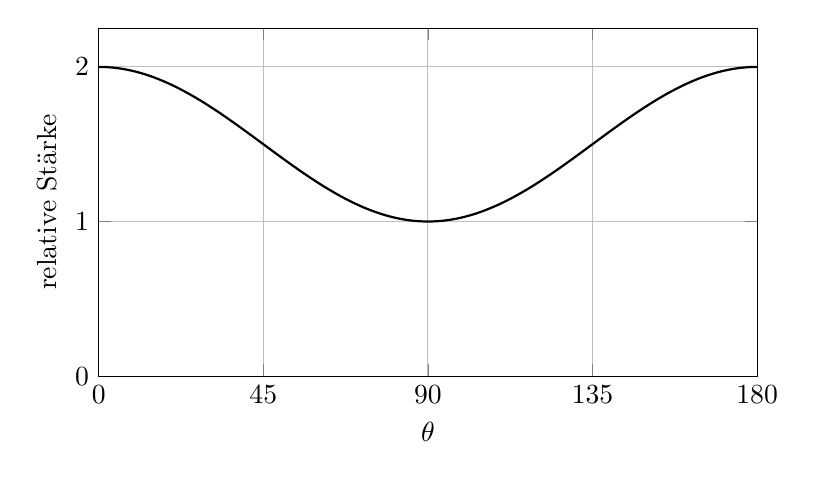
\begin{tikzpicture}
            \begin{axis}[
                width=0.82\textwidth,
                height=6cm,
                xlabel={$\theta$},
                ylabel={relative Stärke},
                xmin=0, xmax=180,
                ymin=0, ymax=2.25,
                xtick={0,45,90,135,180},
                ytick={0,1,2},
                grid=both
            ]
                \addplot[thick,domain=0:180,samples=200]{1+cos(x)^2};
            \end{axis}
        \end{tikzpicture}
        \end{center}
    \end{calculationbox}
\end{enumerate}

\FloatBarrier
\newpage

\section{Aufgabe 2: Titel der Aufgabe}

\begin{definitionbox}
    Eine zentrale Definition oder Annahme, die für mehrere Teilaufgaben gilt.
\end{definitionbox}

\begin{enumerate}[label=(\alph*)]
    \item Weitere Teilaufgabe.
    \begin{solutionbox}
        Hier kann eine ausformulierte Lösung stehen.
    \end{solutionbox}
\end{enumerate}


\end{document}
